\begin{frame}
	\frametitle{Engenharia paraconsistente de características}
	\only<1>{
		\framesubtitle{Os vetores de características proporcionam uma boa separação interclasses?}
		\begin{columns}
		\column{.5\textwidth}				
		\begin{figure}
			\centering
			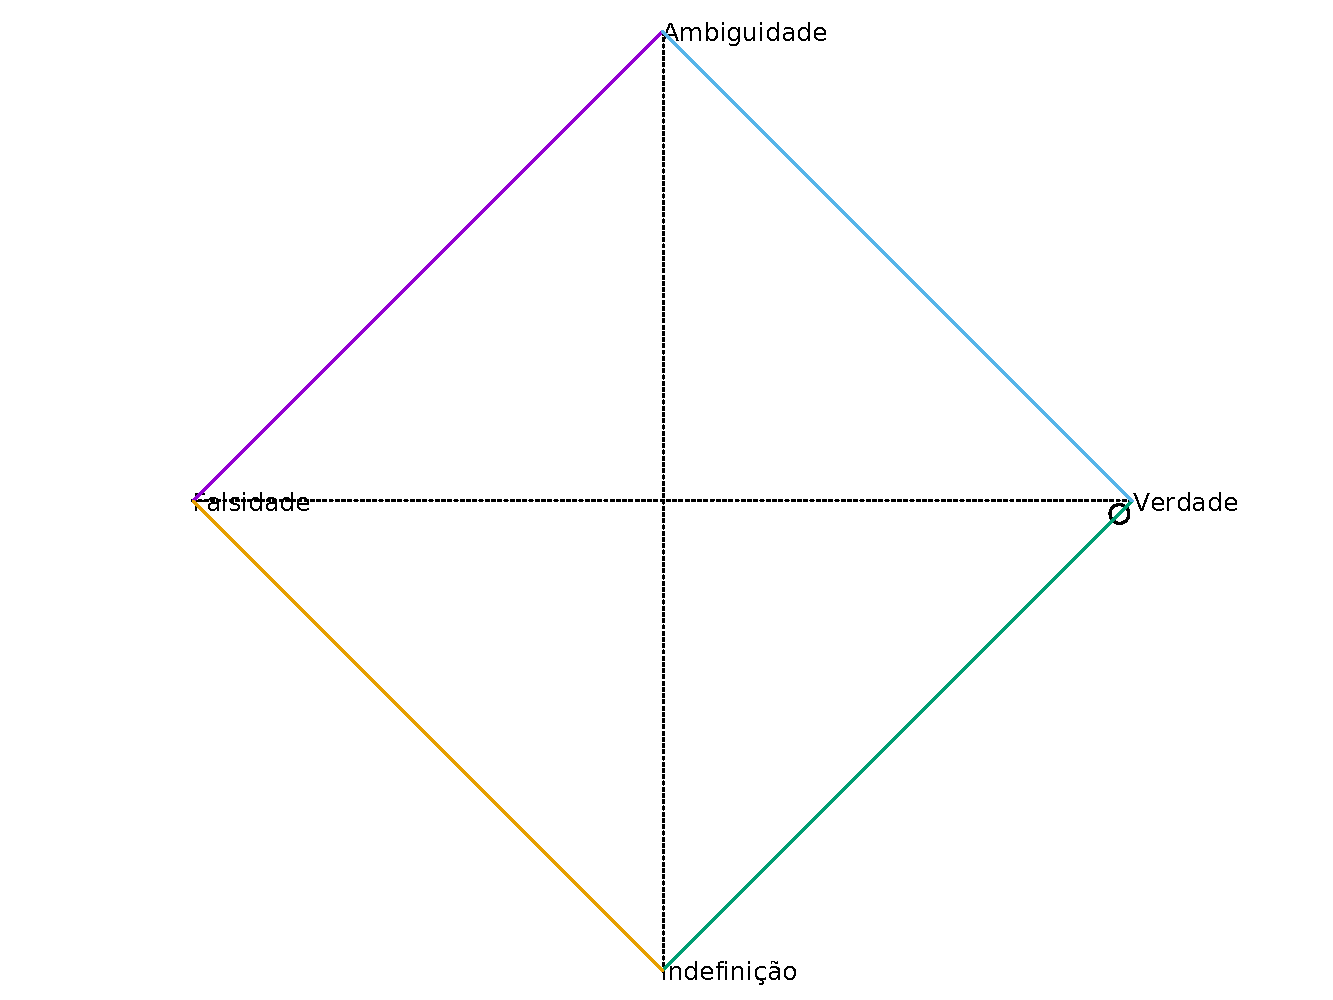
\includegraphics[width=.85\linewidth, angle=-90]{../monography/images/paraconsistentPlane}
			\label{fig:paraconsistentplane}
			\caption{Plano paraconsistente}
		\end{figure}
		\column{.5\textwidth}
		\begin{itemize}
			\item Verdade:\\
		 $\alpha = 1$ e $\beta = 0$.
			\item Ambiguidade:\\
		 $\alpha = 1$ e $\beta = 1$.
			\item Falsidade:\\
		 $\alpha = 0$ e $\beta = 1$.
			\item Indefinição:\\
		 $\alpha = 0$ e $\beta = 0$.
		\end{itemize}
	\end{columns}
	}
	\only<2>{
		\framesubtitle{Cálculo de $\alpha$}
		\begin{columns}
			\column{.5\textwidth}
			\begin{textblock*}{0cm}(.4cm,1.5cm)
				\centering
				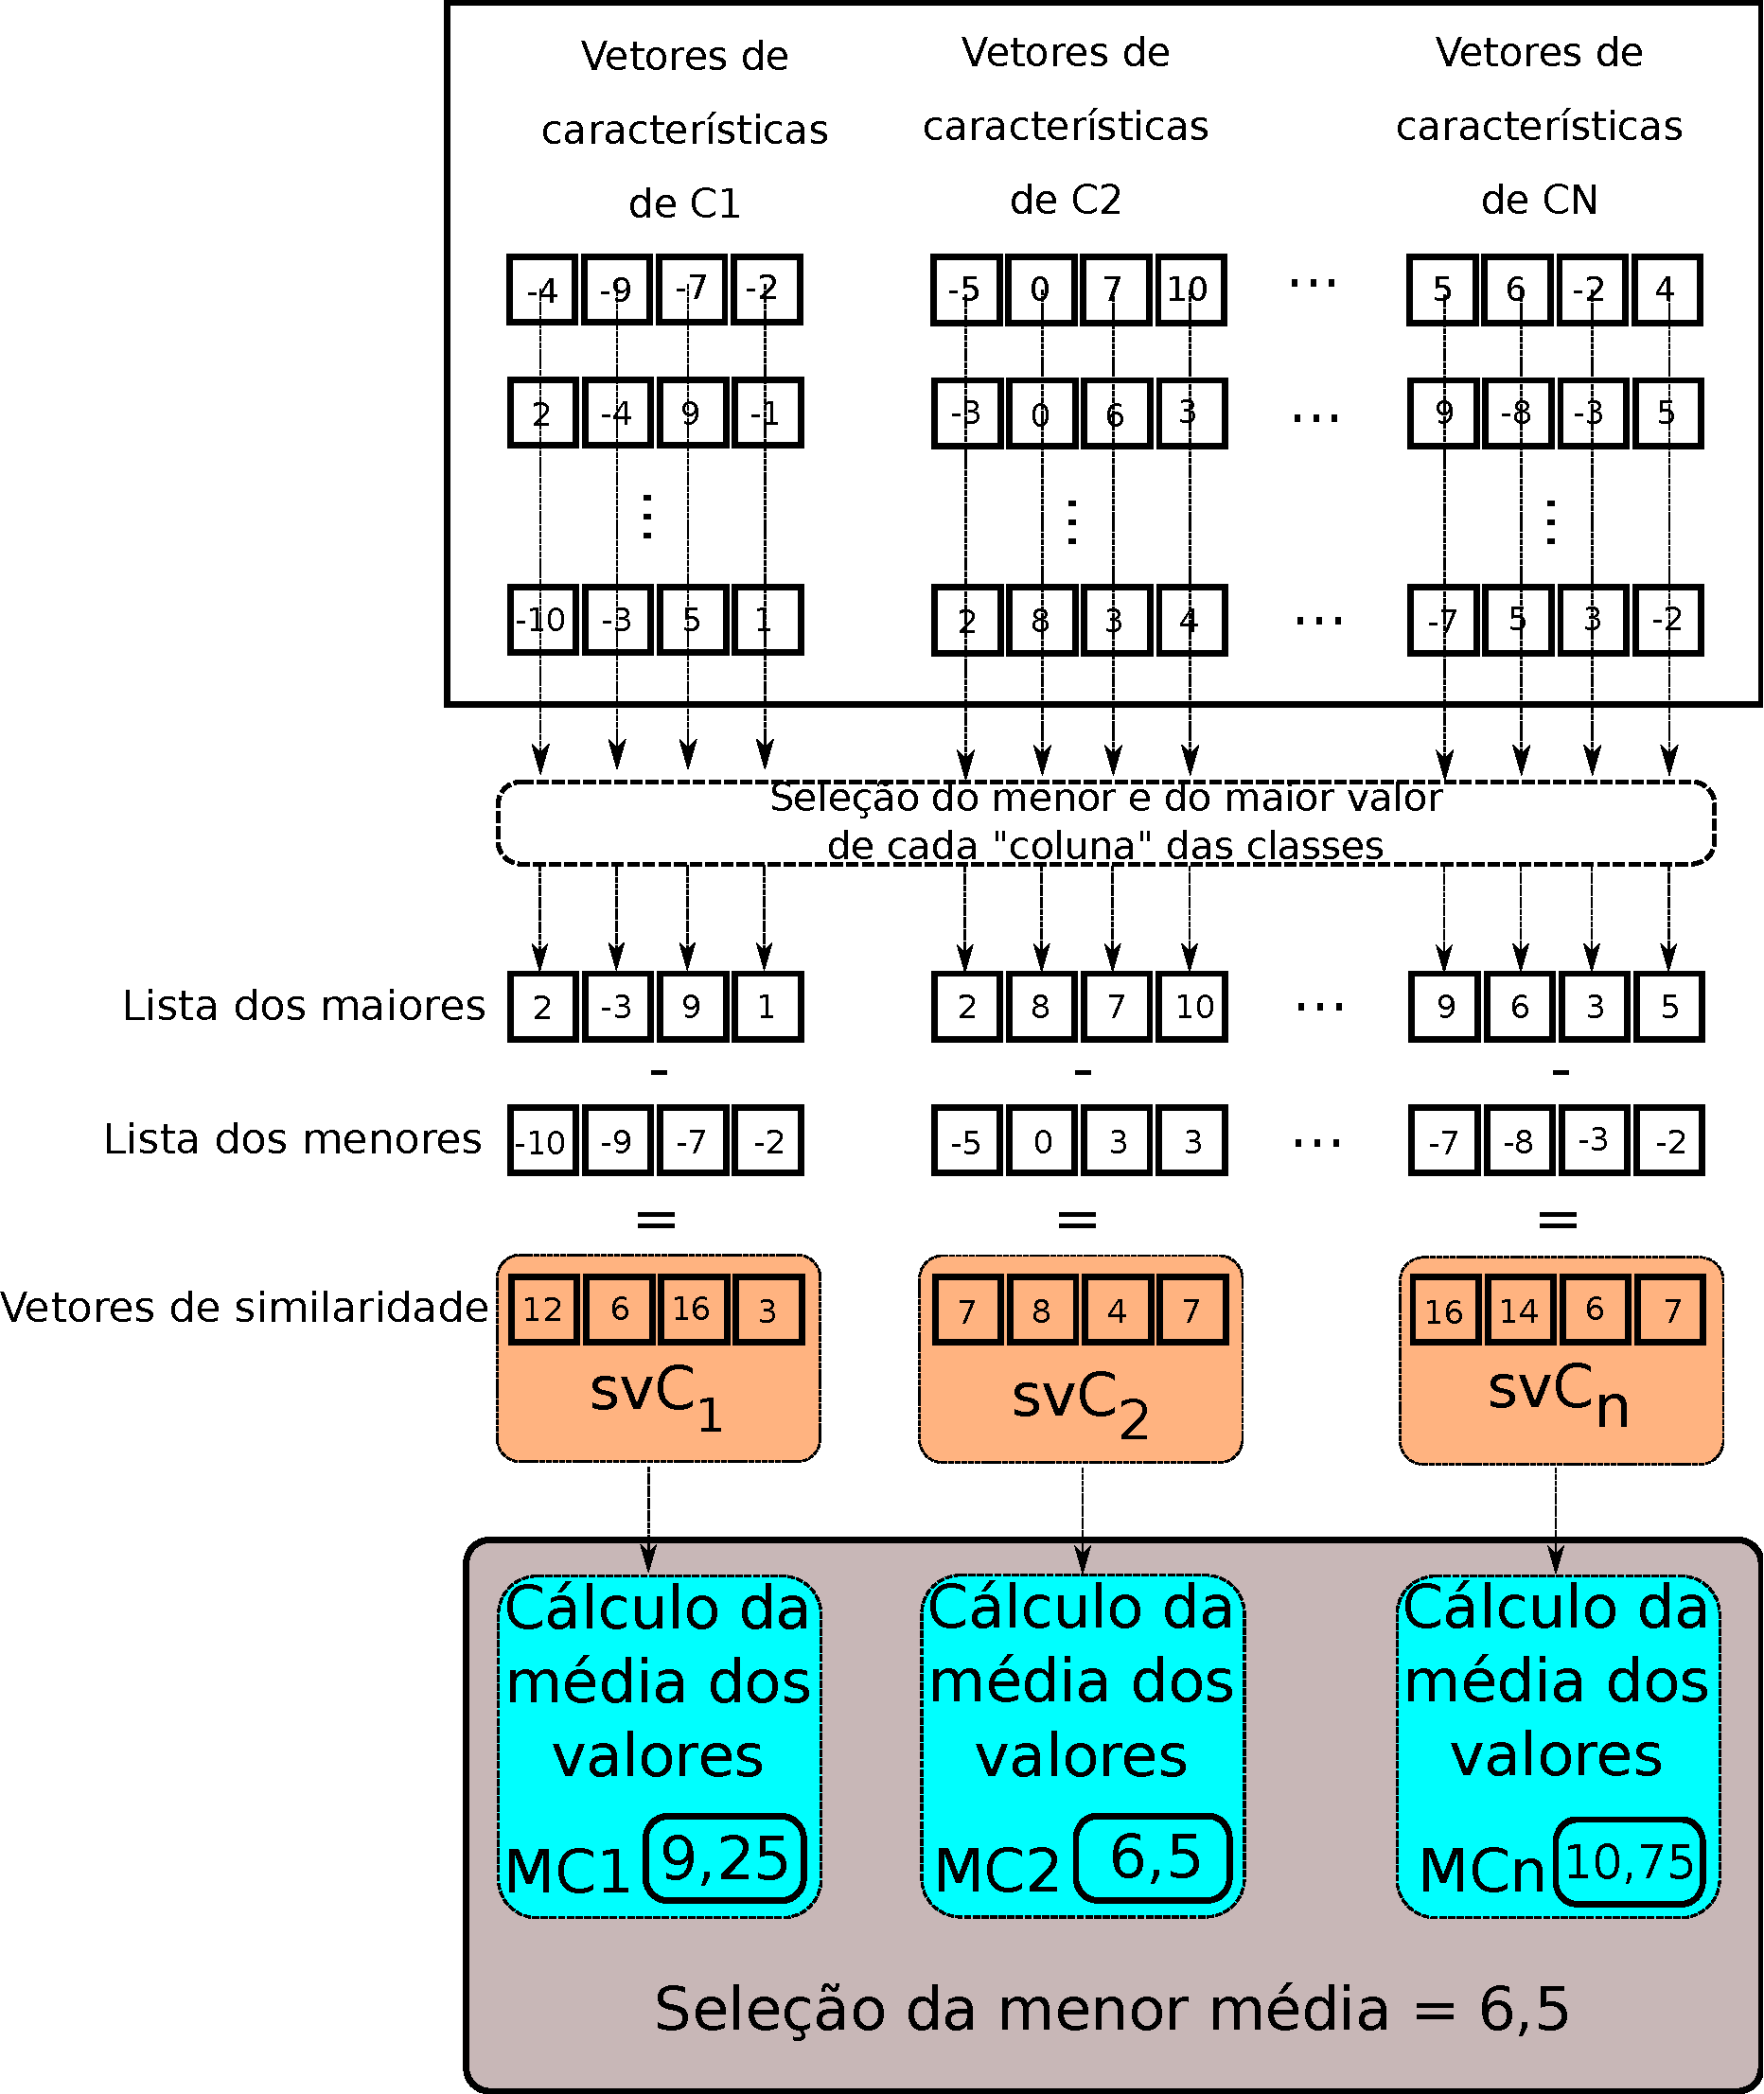
\includegraphics[height=0.82\textheight]{../monography/images/calculoAlpha.pdf}
			\end{textblock*}
			\column{.5\textwidth}
			\par Menor similaridade intraclasse, $\alpha$
		\end{columns}
	}
	\only<3>{
		\framesubtitle{Cálculo de $\beta$}
		\begin{columns}
			\column{.5\textwidth}
			\begin{textblock*}{0cm}(.4cm,1.5cm)
				\centering
				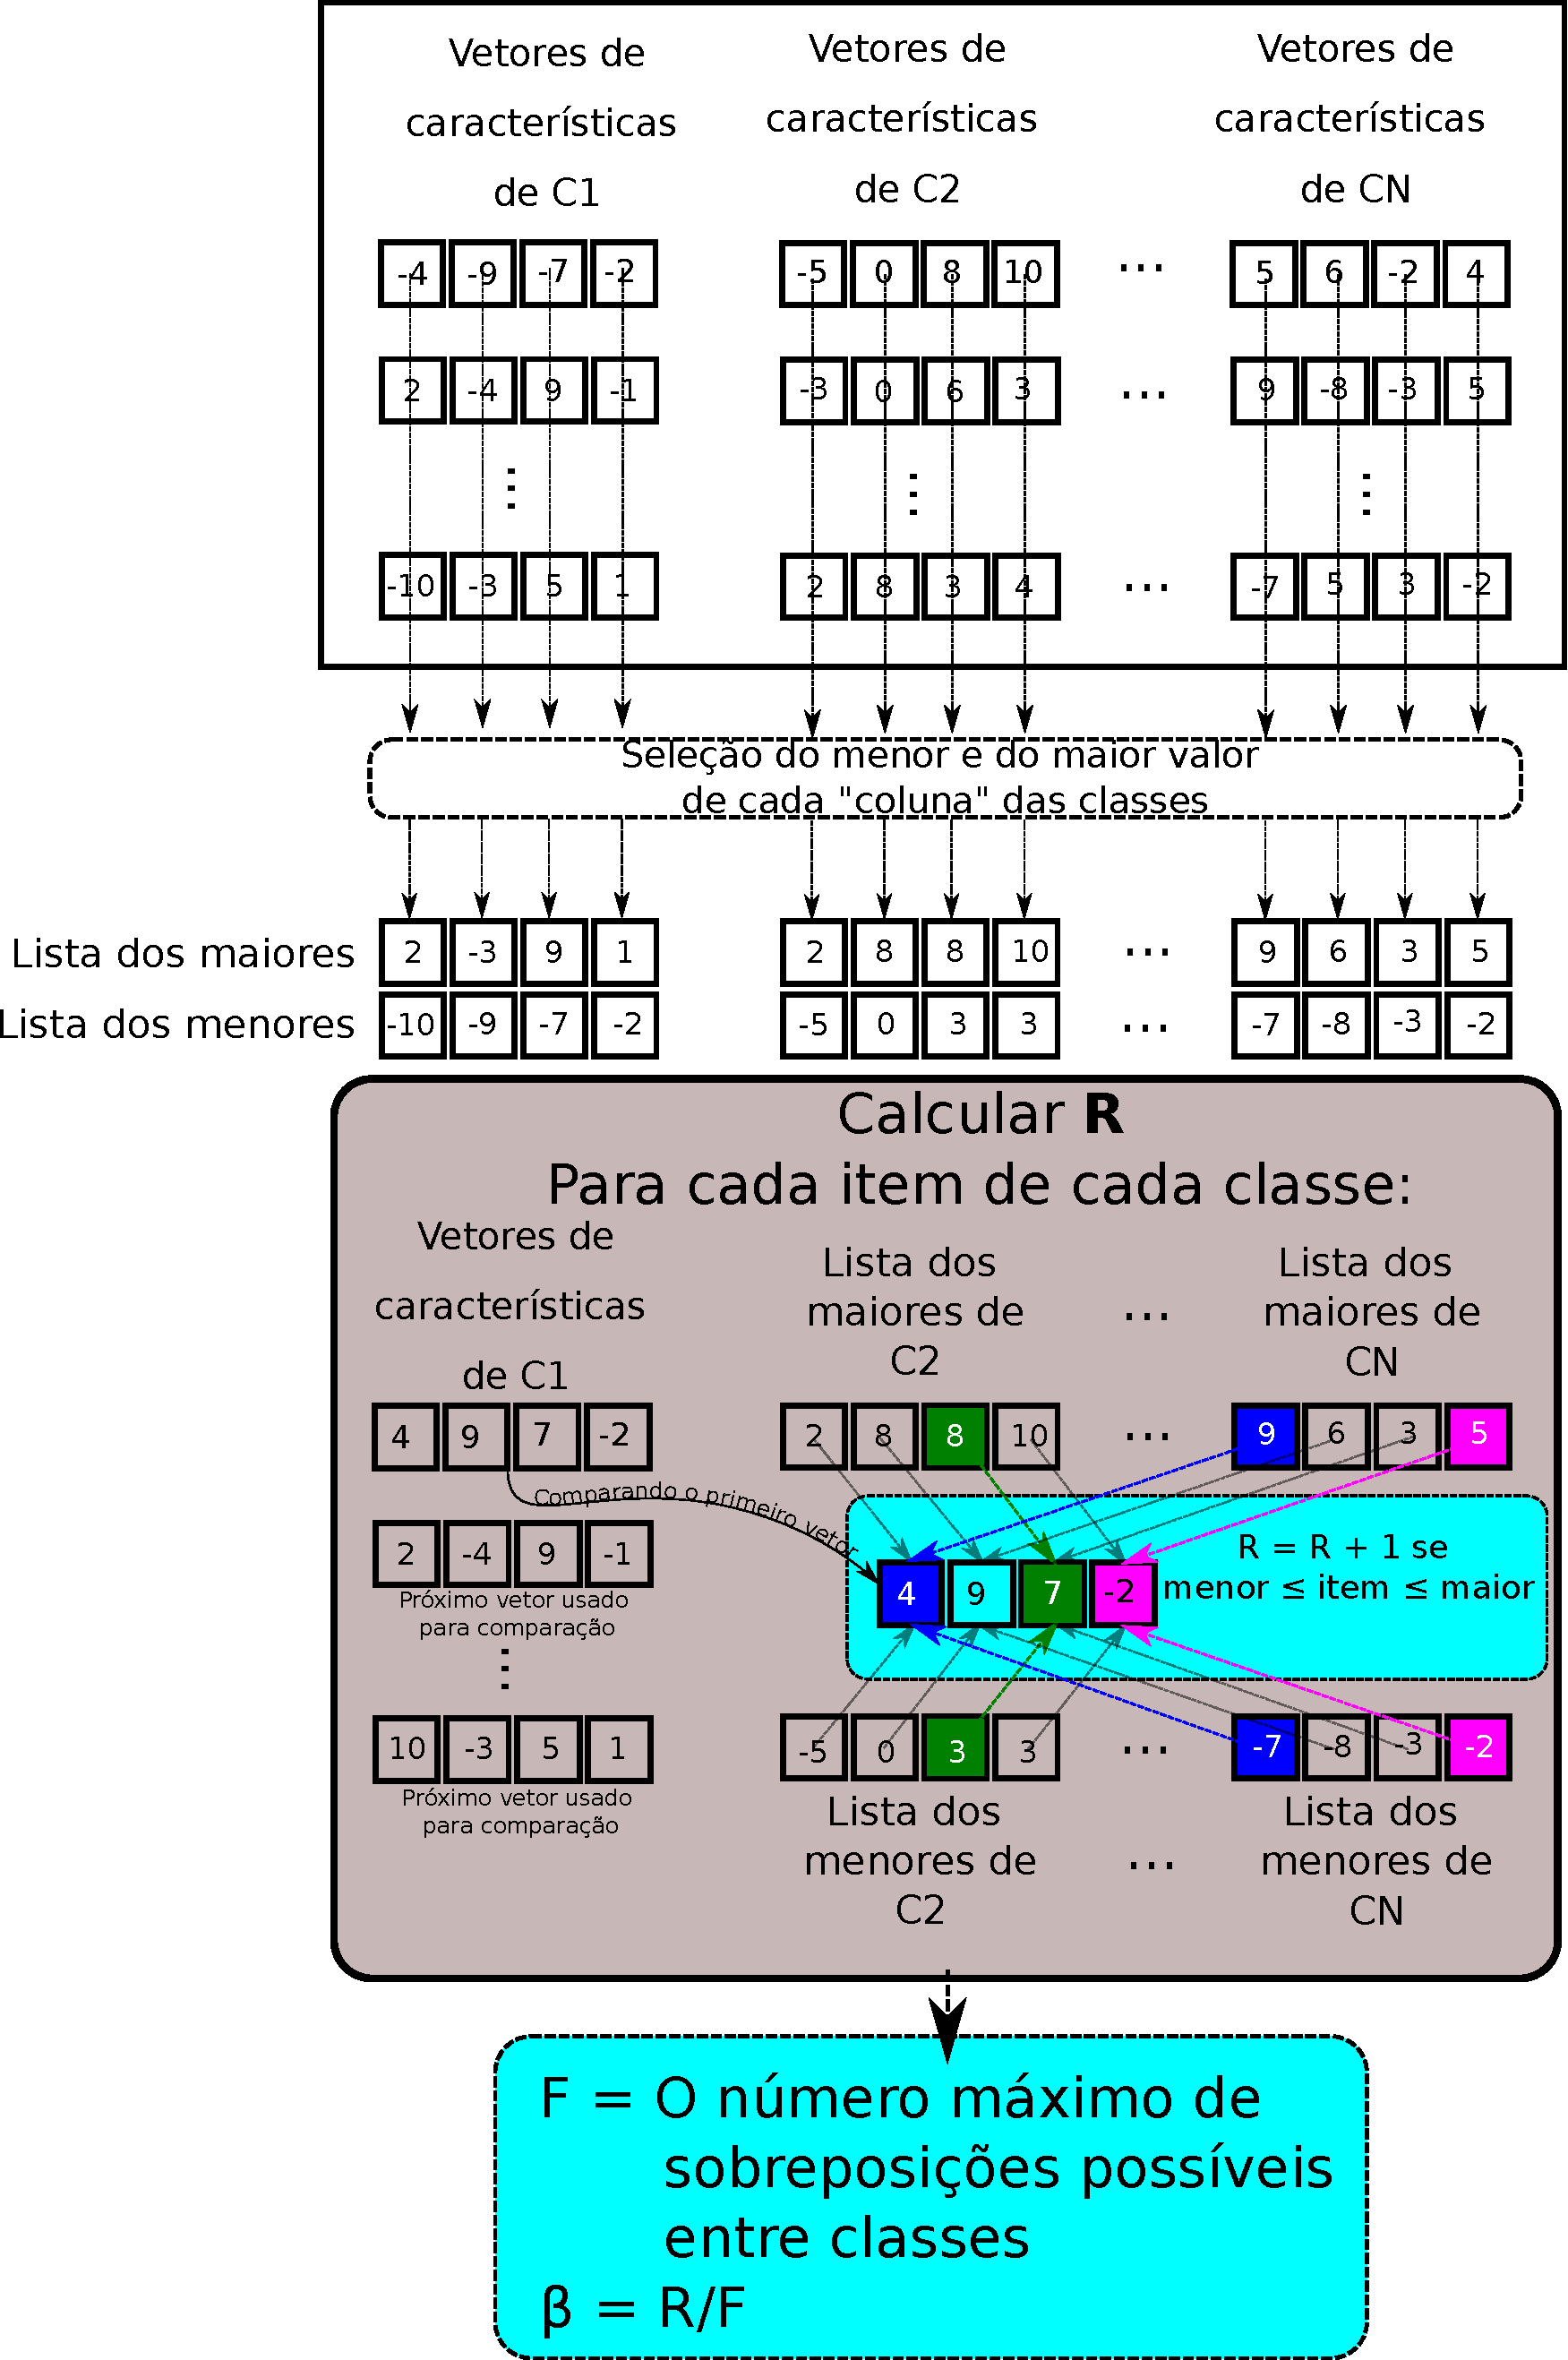
\includegraphics[height=.83\textheight]{../monography/images/betaCalculation.pdf}
			\end{textblock*}
			\column{.5\textwidth}
			\par Razão de sobreposição interclasse, $\beta$.
		\end{columns}
	}
	\only<4>{
		\framesubtitle{Graus de certeza e contradição}
		\begin{itemize}
			\item Grau de certeza $\rightarrow G_1=\alpha-\beta $.
			\item Grau de contradição $\rightarrow G_2=\alpha+\beta-1 $.				
		\end{itemize}
		Onde: $-1 \leqslant G_1 \leqslant 1$ e  $-1 \leqslant G_2 \leqslant 1\qquad$.\\
		Seja $P=(G_1,G_2)$
		\begin{itemize}
			\item (-1,0) $\rightarrow$ Falsidade;
			\item \alert{(1,0) $\rightarrow$ Verdade;}
			\item (0,-1) $\rightarrow$ Indefinição;
			\item (0,1) $\rightarrow$ Ambiguidade.
		\end{itemize}
	}
	\only<5>{
		\framesubtitle{Distancias no plano paraconsistente}
		As distâncias$(D)$ do ponto $P=(G_1,G_2)$ dos limites supracitados. Tal cálculo pode ser feito da seguinte forma:
		\begin{equation*}
		D_{-1,0}=\sqrt{(G_1+1)^2+(G_2)^2}\qquad,
		\end{equation*}
		\alert{
			\begin{equation*}
			D_{1,0}=\sqrt{(G_1-1)^2+(G_2)^2}\qquad,
			\end{equation*}
		}
		\begin{equation*}
		D_{0,-1}=\sqrt{(G_1)^2+(G_2+1)^2}\qquad,		
		\end{equation*}
		\begin{equation*}
		D_{0,1}=\sqrt{(G_1)^2+(G_2-1)^2}\qquad,
		\end{equation*}
	}
\end{frame}